\documentclass[11pt]{article}
\usepackage[margin=1in]{geometry}
\usepackage{authblk}
\usepackage{graphicx}
\usepackage{booktabs}
\usepackage{amsmath, amssymb}
\usepackage{caption}
\captionsetup{font=small,labelfont=bf}
\usepackage{array}
\usepackage[hidelinks]{hyperref}

\title{$\Delta KL$ as an innovation measure for trademark filings:\\
the expected reward to forward flux, and the unexpected reward to
backward flux}
\author{Eric Silver}
\affil{}
\date{May 2026}

\begin{document}
\maketitle

\begin{abstract}
We propose a Kullback--Leibler surprise difference $\Delta KL =
KL_{\text{pros}} - KL_{\text{retr}}$ as an innovation measure for
firm activity, computed on each of $10{,}060{,}073$ U.S.\ trademark
filings in $1990$--$2021$ against per-day exponentially decay-weighted
references of the same NICE class (half-life $H = 2$ years). The
hypothesis going in: filings whose goods/services prose was
\emph{prospectively novel} (unusual against the recent past) and
\emph{retrospectively obvious} (similar to the near future) --- the
trend-setters --- should outperform on post-registration survival,
and $\Delta KL$ should be additive to the standard patent count
proxy. Both predictions are confirmed: conditional on positive
$\Delta KL$, the 4-year stock-return coefficient rises monotonically
through firm-year deciles, and $\Delta KL$ adds explanatory power on
top of $\log(1 + n_\text{patents})$ in the $R^2$ decomposition with
sub-additivity (the two together explain more than either alone
plus the residual). \textbf{The unexpected and unexplained finding}
is that filings at the \emph{opposite} extreme --- prospectively
obvious, retrospectively novel ($\Delta KL < 0$) --- also outperform.
On debut filings the harvest tail is well-fit by a saturating
exponential with $R^2 = 0.978$ on $20$ binned points. The
positive-versus-negative survival lift makes the survival curve
$U$-shaped in $\Delta KL$. The $+U$ holds in $32$ of $44$ NICE
classes; only one industry has a significant inverted-$U$; $11$
indeterminate. We rule out nine alternative explanations and identify
the cluster-viability mediator that absorbs $84\%$ of the quadratic
on survival, leaving a residual linear $\Delta KL$ effect intact.
A long companion paper (\texttt{main.pdf}) reports the per-industry
detail, the financial-outcomes panel, and the per-NICE-class deep
dives.
\end{abstract}

\section{$\Delta KL$ as an innovation measure: the predicted result}

For each filing $i$ at filing-date $t_i$ in NICE class $c$, the
goods/services term distribution $P_i$ is compared via
support-restricted KL divergence to two reference distributions
$Q_i^{\text{pros}}$ and $Q_i^{\text{retr}}$ built by per-day
exponential decay-weighting (half-life $H = 2$ years; the
signal-maximising choice across a sweep of $H \in \{0.5,1,2,3,5\}$
years on Class~9) of all other filings in $c$ before and after
$t_i$ respectively. $\Delta KL_i = KL_i^{\text{pros}} -
KL_i^{\text{retr}}$ is positive when filing $i$'s vocabulary is
unusual against the recent past \emph{and} closer to the near future
--- the directional resonance signal of Murdock, Allen \& DeDeo
(\emph{Cognition}, 2017) applied to commercially incentivised text.
The two component levels are correlated at $\rho = 0.99$ per filing;
the difference is the directional residual.

\paragraph{Hypothesis going in.} Filings at positive $\Delta KL$ ---
prospectively novel and retrospectively obvious --- should outperform
on the standard measures of firm success: registration approval,
post-registration survival, financial returns. $\Delta KL$ should be
\emph{additive} to patent counts, not a noisy redrawing of the same
construct.

\paragraph{Confirmed.} Conditional on positive $\Delta KL$, the
4-year excess-return coefficient over the S\&P~500 is monotone
across firm-year deciles, the firm-debut 4-year excess-return effect
size is approximately $+28$ percentage points per $\sigma$ of
debut $\Delta KL$, and trailing-3-year mean $\Delta KL$ predicts
$+3.2$ pp higher gross margin per $\sigma$ (SE $0.6$ pp) on the
matched SEC-listed firm panel. $\Delta KL$ is essentially uncorrelated
with firm-year patent counts ($r = +0.010$ on $174{,}569$ firm-years)
and \emph{sub-additive} with patent counts in the $R^2$
decomposition: the two predictors together explain more variance
than either alone plus the residual would suggest, indicating they
index distinct innovation channels. Patents proxy a firm's continuing
R\&D output; $\Delta KL$ on the firm's debut filing proxies whether
the firm started in fertile linguistic ground. This is the predicted
result and we treat it as the warm-up; the unexpected finding
follows.

\section{The unexpected finding: the harvest tail also outperforms}

\begin{figure}[t]
\centering
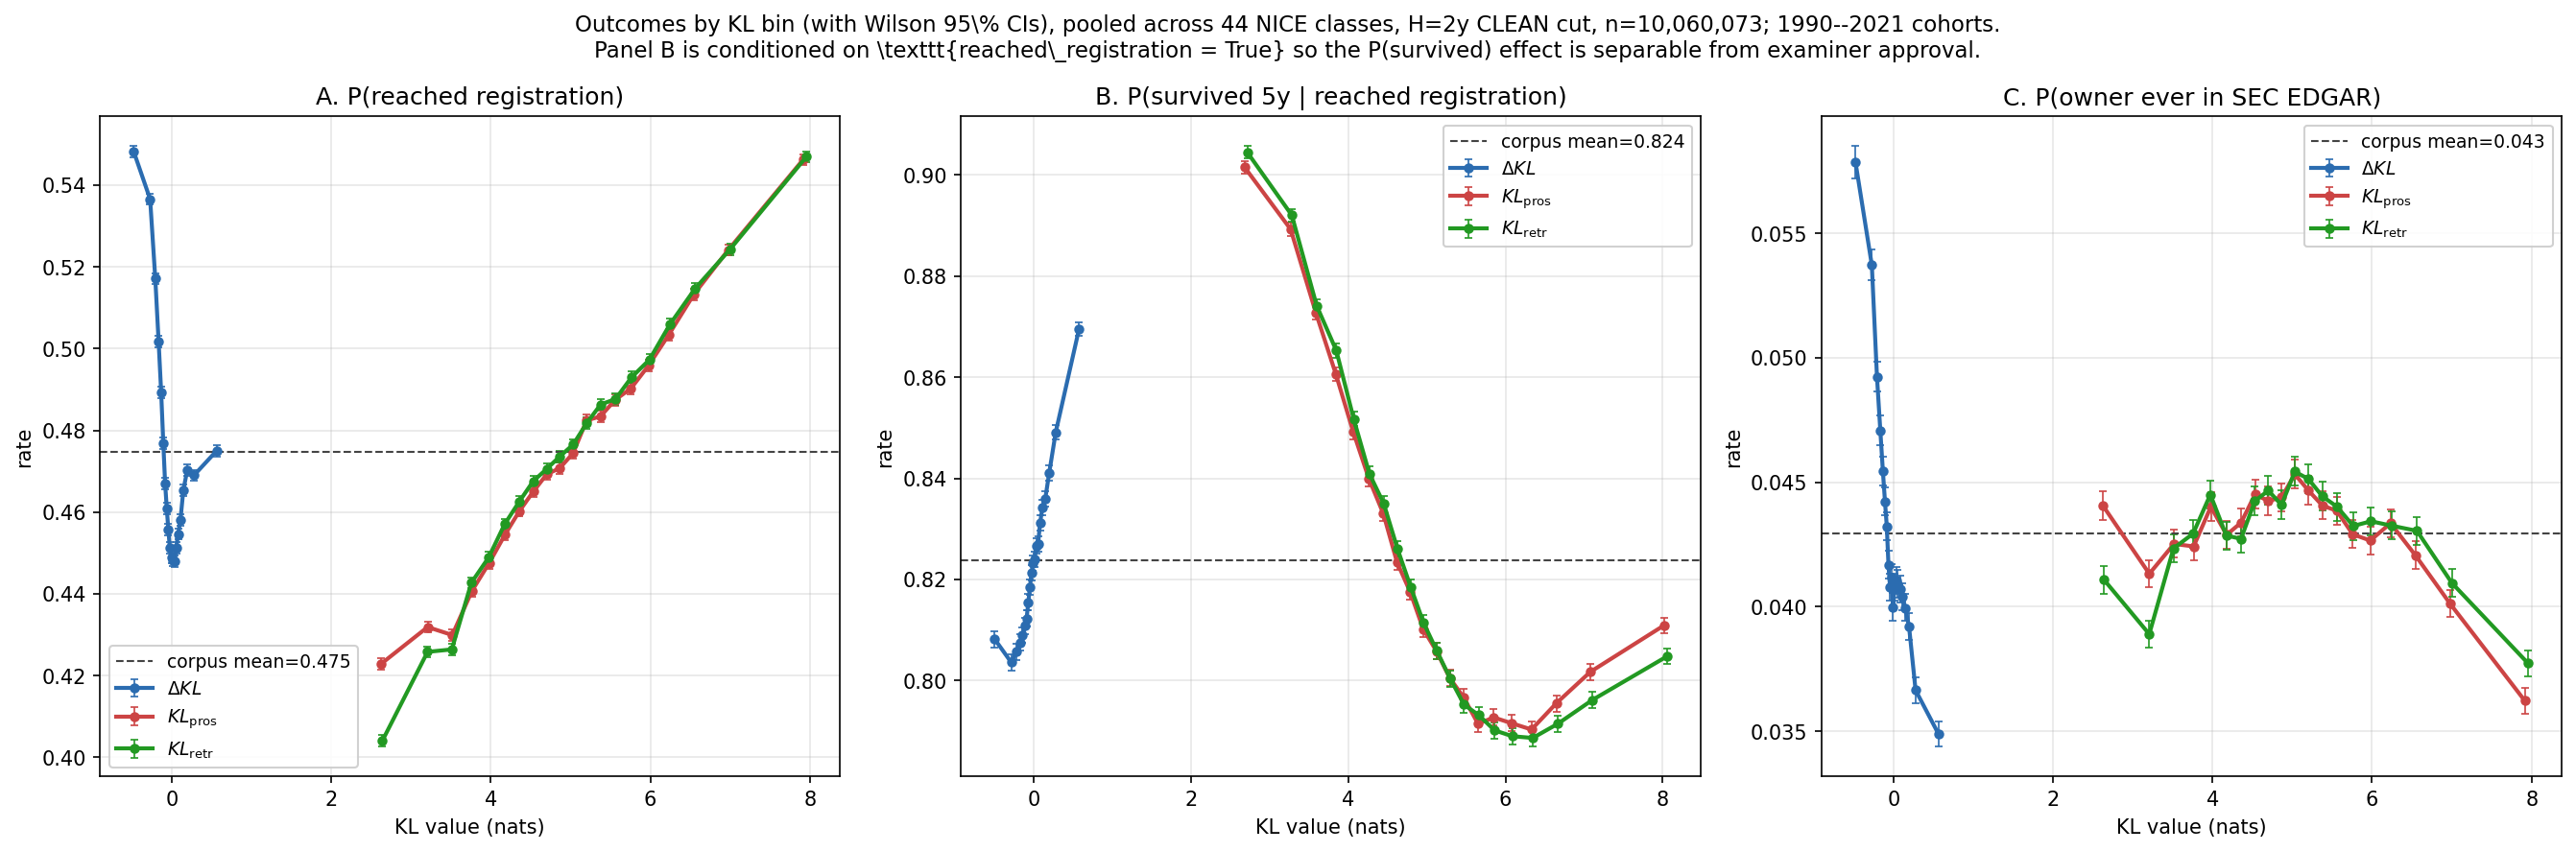
\includegraphics[width=\linewidth]{results/outcome_by_kl_lines_v2.png}
\caption{Three outcomes by KL bin (Wilson 95\% CIs as error bars),
pooled across all $44$ NICE classes; $n = 10{,}060{,}073$ clean
H=2y filings, $1990$--$2021$ cohorts. Panel A: probability the
filing reached registration. \textbf{Panel B: probability the
mark survived $5$ years \emph{conditional on having reached
registration}} (the substantive post-registration mortality
outcome). Panel C: probability the owner ever appears in SEC EDGAR.
On $\Delta KL$ (blue) all three panels show the $U$. On the
component KLs, registration is monotone-up (more-distinctive marks
collide less with prior art and clear examination more easily under
$15$~U.S.C.\ \S\,1052(d)); conditional 5y survival is U-shaped only
on $\Delta KL$, indicating the post-registration mortality
asymmetry is a flux phenomenon and not a distinctiveness phenomenon.}
\label{fig:short-headline}
\end{figure}

Figure~\ref{fig:short-headline} is the central empirical object. The
flux-neutral middle of $\Delta KL$ ($\Delta KL \approx 0$) has the
lowest post-registration $5$-year survival rate in the corpus. Both
extremes outperform it: filings whose vocabulary anticipated where
the field was going (the predicted positive-$\Delta KL$ winners) and
\emph{also} filings whose vocabulary was closer to where the field
had been --- the harvest extreme. We did not predict the harvest
extreme. We do not have a single-mechanism story that explains its
magnitude.

\paragraph{How clean is the harvest tail?} On the debut-filings-only
panel ($n = 5{,}088{,}700$ owner-first filings), we fit a saturating
exponential of survival on $|\Delta KL|$ on each side:
$P(\text{survived}) = a + b\,e^{-c|\Delta KL|}$ on $20$ binned points.
The harvest side (negative $\Delta KL$) fits with $R^2 = 0.978$;
the innovation side (positive $\Delta KL$) fits with $R^2 = 0.499$.
Conditional on negative $\Delta KL$, the correlation between
$|\Delta KL|$ and survival is $+0.054$ (Pearson, $n = 2{,}586{,}126$
debut filings; Spearman $+0.058$). The harvest tail's curve is much
tighter than the innovation tail's; it is doing real work and is
unmistakably present.

\paragraph{The most striking single-token examples of the harvest
tail are in retreating industries.} Negative-$\Delta KL$ tokens that
survive at $50$--$80\%$ in the corpus: \texttt{microfiche},
\texttt{dial-up}, \texttt{pager}, \texttt{store-and-forward},
\texttt{lager}, \texttt{stout}, \texttt{shandy}, \texttt{annuity},
\texttt{microcomputers}. None of these are growing categories; all
support trademarks that the filing firm keeps alive long after the
vocabulary itself recedes from the corpus.

\section{How durable is the $U$? Industry $\times$ year breakdown}

Table~\ref{tab:short-classification} reports the $U$-shape
classification of every $($industry, year$)$ cell in the panel.
For each of $44$ industries with $\geq 5{,}000$ clean filings, we
fit a logistic regression of $5$y survival on $z(\Delta KL)$,
$z(\Delta KL)^2$, and $\log(n_{\text{terms}})$ separately for each
filing-year $1990$--$2021$, and classify the cell by whether the
quadratic coefficient is significantly positive (the $U$), significantly
negative (inverted-$U$), or indeterminate.

\begin{table}[h]
\centering
\small
\begin{tabular}{lrr}
\toprule
Statistic & count & \% of total \\
\midrule
\textbf{Industries (of 44 with sufficient data)} & & \\
  with significant $+U$ on $\Delta KL$ & 32 & 73\% \\
  with significant inverted-$U$ on $\Delta KL$ & 1 & 2\% \\
  indeterminate & 11 & 25\% \\
\midrule
\textbf{Industry $\times$ year cells (of 1,267 total)} & & \\
  significant $+U$ on $\Delta KL$ ($z > +1.96$) & 338 & 27\% \\
  significant inverted-$U$ ($z < -1.96$) & 81 & 6\% \\
  indeterminate quadratic & 848 & 67\% \\
  linear advantage $+\Delta KL$ ($z > +1.96$) & 197 & 16\% \\
  linear advantage $-\Delta KL$ ($z < -1.96$) & 484 & 38\% \\
  neither (linear $|z| \leq 1.96$) & 586 & 46\% \\
\bottomrule
\end{tabular}
\caption{$U$-shape classification of $44$ NICE classes individually
and of the $1{,}267$ $(\text{industry}, \text{year})$ cells where a
logit fit converged. The pooled $+U$ holds in $32$ of $44$ industries;
only $1$ has a significant inverted-$U$ (Telecommunications, where
the linear $\Delta KL$ effect is positive but the harvest tail is
absent). The remaining $11$ are not inverted-$U$ industries --- they
are indeterminate (no significant curvature in either direction).
Cell-level: $27\%$ of cells have a significant $+U$ on $\Delta KL$;
$6\%$ have a significant inverted-$U$; $67\%$ are indeterminate.
Linear-direction counting at the cell level shows a striking
asymmetry: $38\%$ of cells have a significant linear advantage to
\emph{negative} $\Delta KL$ (the harvest direction), versus $16\%$
with significant advantage to positive $\Delta KL$.}
\label{tab:short-classification}
\end{table}

\paragraph{Where does the $U$ not hold and why?} The single
significant inverted-$U$ industry is Telecommunications (NICE 038,
$n = 170{,}826$, $t_{\text{quad}} = -11.8$). It has a positive
linear $\Delta KL$ coefficient ($+0.015$): forward-flux still helps
in telecoms, but the harvest tail is absent --- old telecom
vocabulary does not survive in the way old typesetting or
old-beverage vocabulary does. The $11$ indeterminate industries
split: some (Scientific \& Tech Services $042$, Transport $039$)
have a positive linear coefficient on $\Delta KL$ but neither a
significant quadratic nor a strong harvest tail; others (Hand Tools,
Trim, Jewelry, Vehicles, Ropes \& Textiles, Musical Instruments)
have a \emph{negative} linear coefficient --- mild harvest advantage,
no significant innovation tail to complete the $U$. The interpretation
in both cases is that the industry advantages flux in one direction
but not the other, so the quadratic does not register as
significantly $U$-shaped. None of the $11$ are inverted-$U$
industries where firms in the flux-neutral middle outperform both
extremes.

\section{Nine alternative explanations ruled out; cluster-viability mediates}

Table~\ref{tab:short-falsification} reports the falsification battery
in condensed form. The headline result is that nine alternative
hypotheses for the $U$ are ruled out and a tenth check
(competition-density mediation) identifies the mediator that absorbs
$84\%$ of the quadratic on survival, leaving the linear $\Delta KL$
effect intact.

\begin{table}[h]
\centering
\small
\begin{tabular}{p{4.0cm}p{11.2cm}}
\toprule
\textbf{Alternative} & \textbf{Outcome} \\
\midrule
(1) Foreign-extension artefact (Madrid-Protocol marks) &
Rejected. US-only and foreign-only sub-samples give nearly identical
quadratics ($+0.0078$ and $+0.0100$). \\
\addlinespace
(2) First-time vs.\ recurring filings &
Both have the $U$; recurring slightly stronger. \\
\addlinespace
(3) Same $U$ on financial outcomes &
No. Firm-year gross margin is roughly linear in $\Delta KL$ ($+3.2$ pp/$\sigma$);
the U lives in survival. \\
\addlinespace
(4) Large-incumbent survivor bias on the harvest tail &
Partial. The bottom $\Delta KL$ decile has larger mean firm
filing-volumes than the middle. \\
\addlinespace
(5) ``Liquid Death'' hypothesis (low-$\Delta KL$ is novel products in old vocabulary) &
Rejected on text-length splits. \\
\addlinespace
(6) The $U$ is firm-level (firms with flux-neutral filings just fail) &
Rejected. Within firms that abandoned some marks and kept others
alive (the ``mixed'' cohort, $349{,}819$ firms), the $U$ on
filing-level survival is preserved. \\
\addlinespace
(7) Blockchain / NFT wave as imitated-but-failed counterexample &
Rejected. The crypto cohort outperforms the corpus on every survival
margin. \\
\addlinespace
(8) Vintage pooling artefact &
Rejected. Per-year fits 1990--2021 show the pooled quadratic is
significantly positive in $23$ of $32$ years independently; the $U$
does not track the macro cycle. \\
\addlinespace
(9) English-language usage drift (Google Books n-grams) &
Partial shared signal, not a confound. Per-token correlation between
trademark log-lift and Google Books English log-lift is $+0.47$
($n = 53$). About $22\%$ of trademark-flux variance per token is
shared with general English usage; $78\%$ is corpus-specific. \\
\midrule
\textbf{(10) Competition-density mediation} (the explanation that
sticks) &
$\log(1 + \text{live\_competitors})$ in an asymmetric
$[t-2y,\, t+5y]$ window (cosine $\geq 0.7$ on g/s TF-IDF; not the
H=2y reference window) absorbs $84\%$ of the $\Delta KL$ quadratic
on survival. Flux extremes are in vocabulary clusters where peers
also survive, not in less-competitive clusters. Linear $z(\Delta KL)$
effect remains positive ($z = +2.65$) after the mediator is
included; flux is partly but not wholly redundant with cluster
viability. \\
\bottomrule
\end{tabular}
\caption{Falsification battery for the survival $U$ on $\Delta KL$.
Test (10) is a mediator (it explains most of the shape) rather than
a confound (it doesn't make the shape go away). Long-form treatment
of every test is in Appendix~C of the companion paper.}
\label{tab:short-falsification}
\end{table}

The mediator clarifies the substantive interpretation. Filings at
flux extremes are in vocabulary clusters whose peers can also support
real businesses; the flux-neutral middle is in clusters where peers
are also failing. The survival $U$ is a niche-viability signal
mediated through $\Delta KL$. The linear residual --- ``forward flux
still helps after the mediator is included'' --- is the part of
$\Delta KL$'s information that competition-density alone cannot
reproduce.

\section{What we don't know}

(i) Whether the harvest tail reflects intelligent harvesting (firms
recognising an industry transition and extracting from the legacy
side with their eyes open), passive late-occupation (firms whose
business naturally uses the receding vocabulary because they are
still doing the legacy thing), or selection on something unobservable
(firms surviving long enough to file legacy-vocabulary trademarks
have already proved durable). The trademark record does not
distinguish these.
(ii) Why the linear $z(\Delta KL)$ effect on survival
survives the cluster-viability control. The most plausible
explanation is that conditional on a viable cluster, firms whose
vocabulary moves toward the cluster's future are ahead of firms
whose vocabulary moves against it.
(iii) Whether the firm-level financial reward to flux
($+3.2$ pp gross margin per $\sigma$ of trailing $\Delta KL$ for
public firms; $+28$ pp 4-year excess return per $\sigma$ of debut
$\Delta KL$) is robust to the cluster-viability control. We have
not yet computed the firm-level mediation regression.

The companion paper \texttt{paper/main.pdf} reports the same headline
finding with substantially more apparatus: full per-industry detail
(44 NICE classes worked separately), the financial-outcomes panel on
$\sim 1{,}500$ SEC-listed firms, multi-horizon stock returns analysis
with patent-count controls, the cross-buzzword pioneer-ladder
analysis, the canonical-winner-and-failed-firm KL profile, the
per-industry deep-dive appendix with $44$ scatter plots of public
firms by debut year, and full long-form treatment of all ten
falsification tests in Appendix~C.

\end{document}
